\documentclass[12pt, titlepage]{article}

\usepackage{booktabs}
\usepackage{tabularx}
\usepackage{hyperref}
\usepackage{graphicx}

\hypersetup{
    colorlinks,
    citecolor=black,
    filecolor=black,
    linkcolor=red,
    urlcolor=blue
}
\usepackage[round]{natbib}

\title{SE 3XA3: Software Requirements Specification\\Title of Project}

\author{Team \#, Team Name
		\\ Student 1 Abdallah Taha and tahaa8
		\\ Student 2 name and macid
		\\ Student 3 name and macid
}

\date{\today}

\begin{document}

\maketitle

\pagenumbering{roman}
\tableofcontents
\listoftables
\listoffigures

\begin{table}[bp]
\caption{\bf Revision History}
\begin{tabularx}{\textwidth}{p{3cm}p{2cm}X}
\toprule {\bf Date} & {\bf Version} & {\bf Notes}\\
\midrule
Date 1 & 1.0 & Notes\\
Date 2 & 1.1 & Notes\\
\bottomrule
\end{tabularx}
\end{table}

\newpage

\pagenumbering{arabic}

This document describes the requirements for ....  The template for the Software
Requirements Specification (SRS) is a subset of the Volere
template~\citep{RobertsonAndRobertson2012}.  If you make further modifications
to the template, you should explicity state what modifications were made.

\section{Project Drivers}

\subsection{The Purpose of the Project}

\subsection{The Stakeholders}

\subsubsection{The Client}

\subsubsection{The Customers}

\subsubsection{Other Stakeholders}

\subsection{Mandated Constraints}

\subsection{Naming Conventions and Terminology}

\subsection{Relevant Facts and Assumptions}

User characteristics should go under assumptions.

\section{Functional Requirements}

\subsection{The Scope of the Work and the Product}

\subsubsection{The Context of the Work}

A web browser application which contains the game Tetris. This software product will be able to recognize block patterns that complete a consecutive row on a grid. This application will also contain a scoring system based on length of game time as well as points received from completing a row on the grid. The software will also recognize when the stacked blocks reach a level above the maximum grid and will in turn end the game. Our program will also have different difficulty options that will change the speed at which the blocks fall onto the grid. 

\subsubsection{Work Partitioning}
The backend of the project will be responsible for the game mechanics as well as the scoring and difficulty settings. For the game mechanics the backend software will be responsible for creating a grid for the playable area. It will also generate random blocks from a set list of available blocks; these blocks will then drop down onto the grid and the user will have access to rotate the block 360 degrees in 90-degree increments until it lands on a pre-existing block within the grid. The backend of the software will also need to keep track of the score of the game based on when a row in the grid is filled with blocks, it will then remove the blocks in that row from the grid. Finally, the backend will also be responsible for the different difficulties In the game and will change the speed of the blocks falling onto the grid based on the user selected difficulty. The frontend of the project is responsible for displaying the blocks and the grid as well as showing the current score of the game and the chosen difficulty. It will also have a start button and difficulty button that a user must press and choose in order to start the game. 

\subsubsection{Individual Product Use Cases}

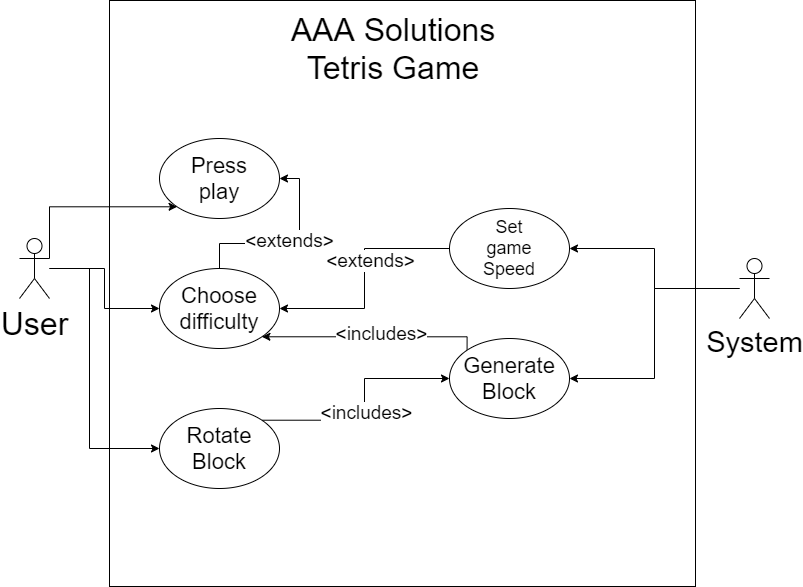
\includegraphics[width=0.95\linewidth]{usecasexa3.png}

\subsection{Functional Requirements}

\section{Non-functional Requirements}

\subsection{Look and Feel Requirements}

\subsection{Usability and Humanity Requirements}

\subsection{Performance Requirements}

\subsection{Operational and Environmental Requirements}

\subsection{Maintainability and Support Requirements}

\subsection{Security Requirements}

\subsection{Cultural Requirements}

\subsection{Legal Requirements}

\subsection{Health and Safety Requirements}

This section is not in the original Volere template, but health and safety are
issues that should be considered for every engineering project.

\section{Project Issues}

\subsection{Open Issues}

\subsection{Off-the-Shelf Solutions}

\subsection{New Problems}

\subsection{Tasks}

\subsection{Migration to the New Product}

\subsection{Risks}

\subsection{Costs}

\subsection{User Documentation and Training}

\subsection{Waiting Room}

\subsection{Ideas for Solutions}

\bibliographystyle{plainnat}

\bibliography{SRS}

\newpage

\section{Appendix}

This section has been added to the Volere template.  This is where you can place
additional information.

\subsection{Symbolic Parameters}

The definition of the requirements will likely call for SYMBOLIC\_CONSTANTS.
Their values are defined in this section for easy maintenance.


\end{document}